\chapter{Estado da Arte}
\label{cap:estado_da_arte}

O desenvolvimento de um painel de administração, também designado por \textit{backoffice}, exige uma análise diferente da que seria feita para uma aplicação pública. Estes sistemas são utilizados por operadores internos, têm acesso restrito e, por isso, raramente disponibilizam publicamente todos os seus fluxos, ecrãs e regras de funcionamento. Esta limitação condiciona a análise de trabalhos relacionados: em vez de procurar apenas produtos equivalentes com demonstrações completas, torna-se mais adequado estudar padrões observáveis em painéis de administração, ferramentas de construção de aplicações internas e recomendações técnicas para autorização e auditoria.

No caso deste projeto, o \textit{backoffice} foi também concebido como uma base multiaplicação. No estado atual, existem o módulo transversal de administração dos próprios operadores, perfis e permissões do \textit{backoffice}, e a aplicação JustCauses como primeiro domínio funcional. Ainda assim, a estrutura foi desenhada para facilitar a integração futura de outras aplicações no mesmo painel, reutilizando autenticação, controlo de acesso, auditoria e navegação base.

Para apoiar a identificação inicial de exemplos públicos, foram usados mecanismos de pesquisa automática orientados pelos critérios definidos neste capítulo; a seleção final privilegiou apenas os casos com informação pública suficiente e relevância direta para o projeto.

Neste capítulo analisam-se, primeiro, as capacidades mais relevantes para um painel de administração seguro e auditável. Em seguida, apresentam-se sistemas e ferramentas relacionados, dando autonomia a cada exemplo analisado. Por fim, enquadram-se as tecnologias usadas no projeto, separando as escolhas já existentes na empresa das decisões relevantes para o trabalho desenvolvido durante o estágio.

%----------------------------------------------------------------------------------------

\section{Critérios de análise}
\label{sec:criterios_analise}

O painel desenvolvido neste estágio não corresponde a uma aplicação de consumidor final. O seu objetivo é apoiar operações internas do ecossistema OnlyHighIQ, começando pela administração transversal do próprio \textit{backoffice} e pela aplicação JustCauses. Assim, a análise do estado da arte deve privilegiar critérios ligados à operação, à segurança e à evolução multiaplicação, e não apenas aspetos visuais ou escolhas genéricas de \textit{front-end}.

A Tabela~\ref{tab:criterios_backoffice} apresenta os critérios usados para comparar os sistemas e ferramentas analisados neste capítulo.

\begin{table}[H]
\caption{Critérios de análise para painéis de administração}
\label{tab:criterios_backoffice}
\begin{center}
\small
\begin{tabular}{|p{3.4cm}|p{9.2cm}|}
\hline
\textbf{Critério} & \textbf{Relevância para o projeto} \\ \hline
Controlo de acesso & O painel deve distinguir operadores, perfis, aplicações, páginas e ações, aplicando permissões no \textit{front-end} e no \textit{back-end}. \\ \hline
Auditoria & As operações sensíveis devem deixar registos consultáveis, com identificação do operador, ação executada, entidade afetada e data. \\ \hline
Fluxos operacionais & O sistema deve suportar processos internos, como revisão de campanhas, gestão de categorias, consulta financeira e administração de acessos. \\ \hline
Expansão do painel & O painel deve permitir a integração futura de novas aplicações, reutilizando autenticação, operadores, perfis, permissões, auditoria e navegação base. \\ \hline
Adaptação ao domínio & A solução deve acomodar regras específicas de cada aplicação, como a JustCauses, sem comprometer o núcleo comum do ecossistema da OnlyHighIQ. \\ \hline
Manutenibilidade & A arquitetura deve permitir evolução incremental, testes e integração com a base de código existente. \\ \hline
\end{tabular}
\end{center}
\end{table}

Estes critérios são também coerentes com recomendações de segurança aplicacional. A OWASP recomenda que a autorização seja aplicada no servidor e que o sistema negue o acesso por omissão quando não exista uma regra explícita de permissão \cite{OWASPAuthorizationCheatSheet}. Além disso, o modelo \gls{RBAC} usado no projeto aproxima-se de abordagens mais contextuais quando combina perfil, aplicação, página e ação. Esta ideia é compatível com a definição de controlo de acesso baseado em atributos descrita pelo NIST, onde a autorização resulta da avaliação de atributos do sujeito, do objeto, da operação e, quando aplicável, do contexto \cite{NISTABAC}.

%----------------------------------------------------------------------------------------

\section{Trabalhos relacionados}
\label{sec:trabalhos_relacionados}

A análise de trabalhos relacionados considera exemplos concretos de painéis comerciais e ferramentas de administração configuráveis. Os painéis comerciais permitem observar padrões de operação, permissões e rastreabilidade em produtos consolidados. As ferramentas configuráveis ajudam a avaliar se faria sentido adotar uma solução pronta em vez de uma implementação à medida. Em ambos os casos, a análise é limitada pela disponibilidade pública de informação, uma vez que muitos fluxos de \textit{backoffice} são reservados a equipas internas ou a clientes autenticados.

\subsection{Shopify Admin}
\label{subsec:shopify_admin}

O Shopify Admin é o painel de administração da plataforma Shopify. A sua relevância para este trabalho não está no domínio de comércio eletrónico em si, mas na forma como organiza tarefas operacionais num único ambiente: gestão de produtos, encomendas, clientes, pagamentos, relatórios e acessos de equipa. Esta centralização é útil como referência para sistemas em que diferentes perfis internos executam tarefas distintas no mesmo painel.

A documentação pública descreve um modelo de permissões associado a funções, com permissões ao nível da loja, organização e ponto de venda, dependendo do contexto e do plano contratado \cite{ShopifyStaffAccess}. A Figura~\ref{fig:shopify_admin} apresenta uma vista do Shopify Admin orientada à gestão de encomendas, exemplificando a organização de informação operacional em tabelas, filtros e ações de detalhe.

\begin{figure}[H]
\centering
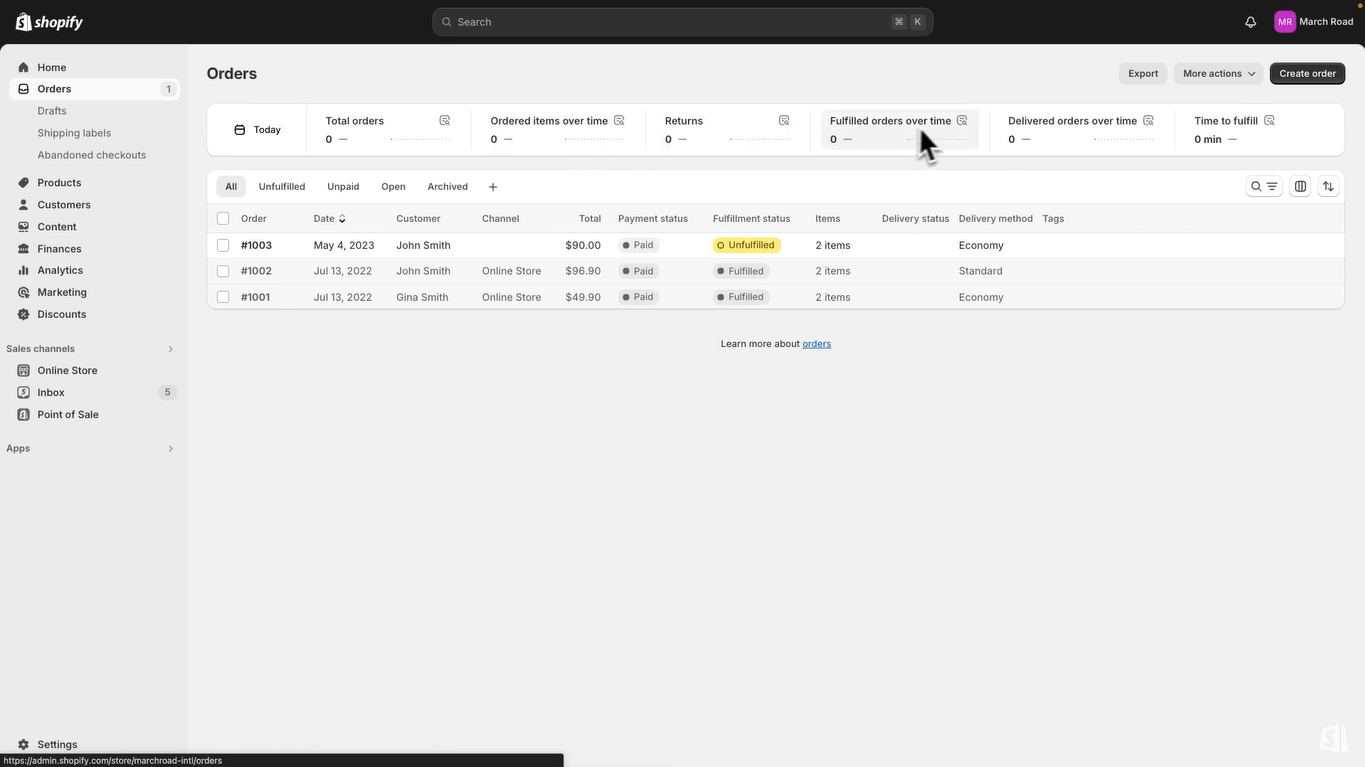
\includegraphics[width=1\textwidth]{frontmatter/assets/backoffice/ch2/shopify_admin.png}
\caption{Interface de gestão de encomendas do Shopify Admin \cite{ShopifyAbout}}
\label{fig:shopify_admin}
\end{figure}

\paragraph{Contributos para o projeto}
\begin{itemize}
  \item Separação clara entre áreas funcionais e ações sensíveis.
  \item Utilização de perfis e permissões para limitar operações por tipo de utilizador interno.
  \item Organização de listagens, filtros e vistas de detalhe para tarefas recorrentes.
\end{itemize}

\paragraph{Limitações}
\begin{itemize}
  \item Domínio fortemente orientado a comércio eletrónico, sem correspondência direta com todos os fluxos do painel desenvolvido.
  \item Produto fechado, sem acesso à arquitetura interna ou possibilidade de reutilização estrutural.
  \item Informação pública limitada sobre auditoria detalhada de ações de operadores.
\end{itemize}

\subsection{Stripe Dashboard}
\label{subsec:stripe_dashboard}

O Stripe Dashboard é o painel de administração da Stripe para acompanhamento de pagamentos, disputas, reembolsos, eventos e membros de equipa. É uma referência relevante para operações financeiras, porque apresenta informação sensível com histórico, filtros e detalhe suficiente para apoiar decisões operacionais.

A documentação da Stripe descreve a atribuição de funções a membros da equipa, a possibilidade de um utilizador acumular vários papéis e a existência de histórico de segurança com atividade dos membros da conta \cite{StripeTeams}. As funções específicas do Stripe Identity, como \textit{Identity Analyst} e \textit{Identity View Only}, mostram uma separação operacional entre consulta e revisão de verificações de identidade \cite{StripeUserRoles}. A Figura~\ref{fig:stripe_dashboard} ilustra uma vista de gestão de transações, relevante para compreender como um painel financeiro apresenta estados, valores e ações associadas.

\begin{figure}[H]
\centering
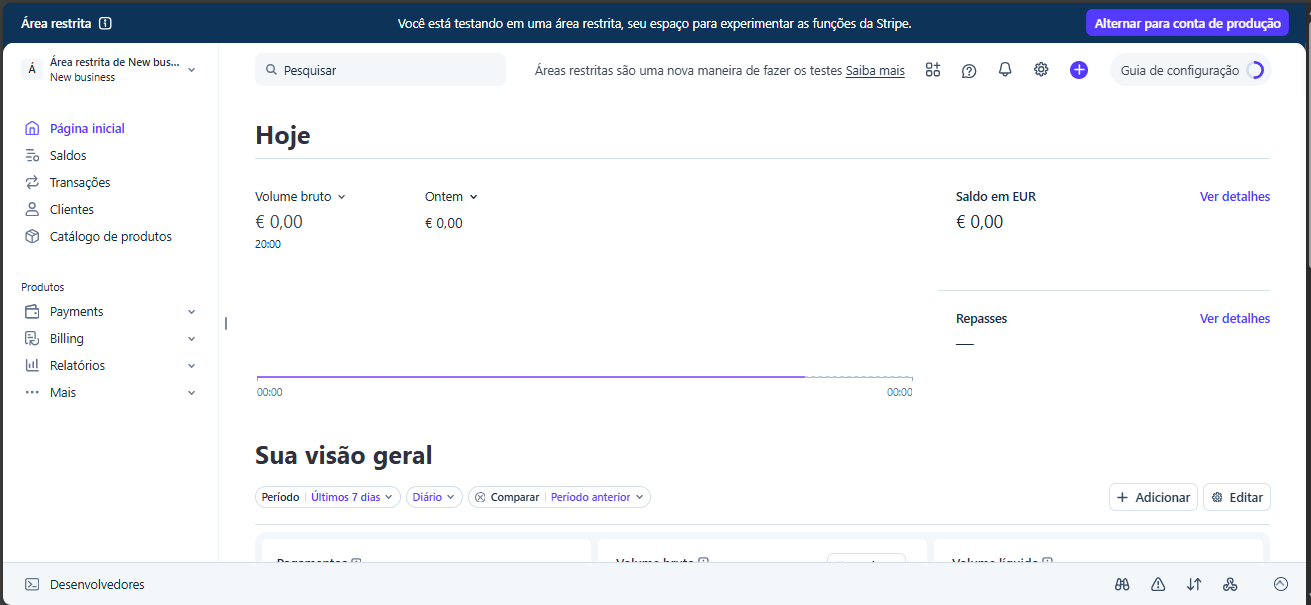
\includegraphics[width=1\textwidth]{frontmatter/assets/backoffice/ch2/stripe_dashboard.png}
\caption{Interface de gestão de transações do Stripe Dashboard \cite{StripeDashboard}}
\label{fig:stripe_dashboard}
\end{figure}

\paragraph{Contributos para o projeto}
\begin{itemize}
  \item Separação de permissões por tipo de operação financeira.
  \item Histórico de atividade associado a membros da conta.
  \item Apresentação de transações com estados, filtros e detalhe operacional.
\end{itemize}

\paragraph{Limitações}
\begin{itemize}
  \item Foco específico no domínio financeiro, sem cobertura de outros fluxos administrativos.
  \item Produto fechado, não adaptável a regras de negócio externas.
  \item A documentação pública descreve conceitos de utilização, mas não a implementação interna do painel.
\end{itemize}

\subsection{Directus}
\label{subsec:directus}

O Directus representa uma abordagem orientada a dados. A ferramenta disponibiliza uma interface de administração sobre bases de dados existentes e permite definir permissões por coleção, ação, campo e política \cite{DirectusPermissions}. Esta granularidade torna o Directus relevante para sistemas em que a principal necessidade é consultar e alterar entidades persistidas.

A Figura~\ref{fig:directus} apresenta uma interface de gestão de dados do Directus. A estrutura evidencia uma lógica comum em ferramentas deste tipo: o modelo de dados serve de base à interface, e a administração é organizada em torno de coleções, campos e operações.

\begin{figure}[H]
\centering
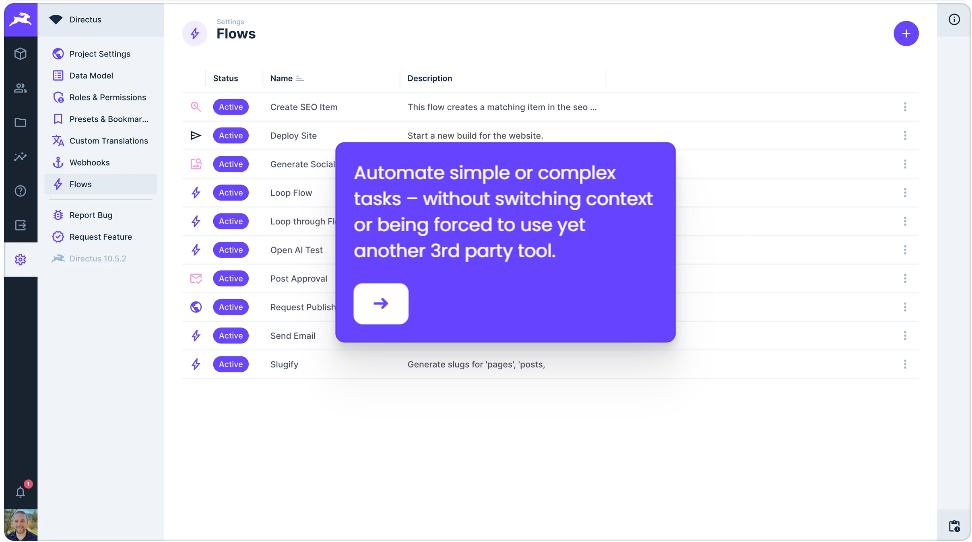
\includegraphics[width=1\textwidth]{frontmatter/assets/backoffice/ch2/directus.png}
\caption{Interface de gestão de dados do Directus \cite{DirectusAbout}}
\label{fig:directus}
\end{figure}

\paragraph{Contributos para o projeto}
\begin{itemize}
  \item Permissões granulares por entidade, campo e ação.
  \item Administração rápida de dados existentes sem desenvolver todas as vistas manualmente.
  \item Registo de atividade e configuração centralizada de regras de acesso.
\end{itemize}

\paragraph{Limitações}
\begin{itemize}
  \item Interface construída a partir do modelo de dados, menos adequada a fluxos de negócio com estados e validações próprias.
  \item Necessidade de configuração ou desenvolvimento adicional para processos de aprovação específicos.
  \item Dependência da forma como as entidades estão modeladas na base de dados.
\end{itemize}

\subsection{Appsmith}
\label{subsec:appsmith}

O Appsmith segue uma abordagem \textit{low-code} para criação de ferramentas internas. A documentação descreve a ligação a bases de dados e \glspl{API}, a construção de interfaces com componentes visuais e a escrita de lógica através de consultas e JavaScript \cite{AppsmithDocs}. Esta solução é relevante porque mostra uma alternativa à criação manual de um painel completo, sobretudo em contextos de prototipagem ou de ferramentas internas de baixa complexidade.

A Figura~\ref{fig:appsmith} mostra a construção visual de uma ferramenta interna no Appsmith, com componentes de interface ligados a fontes de dados. Esta abordagem reduz o tempo inicial de desenvolvimento, mas desloca parte da lógica para configurações e scripts dentro da própria ferramenta.

\begin{figure}[H]
\centering
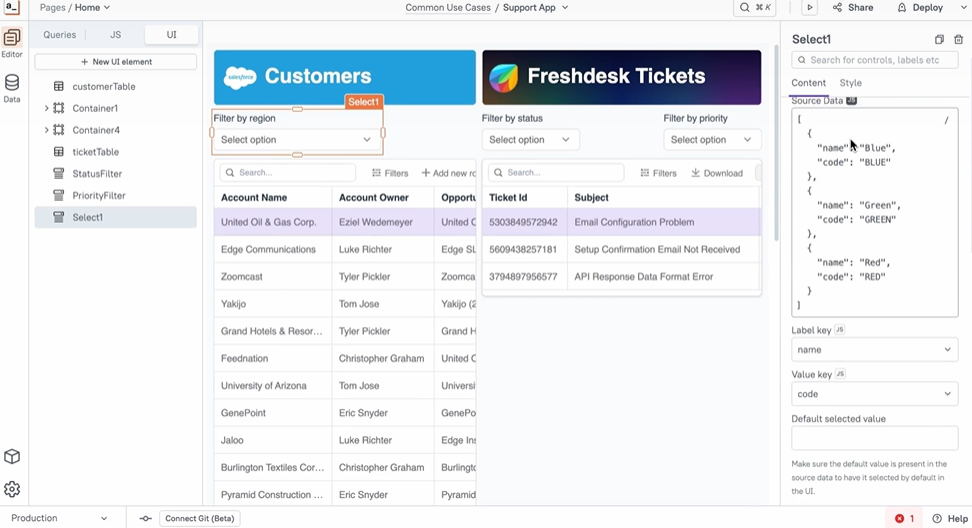
\includegraphics[width=1\textwidth]{frontmatter/assets/backoffice/ch2/appsmith.png}
\caption{Interface de construção de ferramentas internas no Appsmith \cite{AppsmithAbout}}
\label{fig:appsmith}
\end{figure}

\paragraph{Contributos para o projeto}
\begin{itemize}
  \item Criação rápida de interfaces internas ligadas a dados e \glspl{API}.
  \item Adequação a protótipos e painéis operacionais de baixa complexidade.
  \item Redução do esforço inicial em formulários, tabelas e ligações a fontes de dados.
\end{itemize}

\paragraph{Limitações}
\begin{itemize}
  \item Lógica de negócio distribuída por componentes e scripts, com impacto na testabilidade.
  \item Menor controlo sobre a arquitetura da aplicação quando comparado com uma implementação própria.
  \item Adequação limitada a fluxos sensíveis que exigem auditoria consistente e validação transversal no servidor.
\end{itemize}

\subsection{Análise comparativa}
\label{subsec:analise_comparativa_backoffices}

A Tabela~\ref{tab:comparacao_abordagens_backoffice} sintetiza os exemplos analisados e a sua relevância para o projeto, usando a abordagem apenas como uma característica de enquadramento.

\begin{table}[H]
\caption{Comparação de exemplos de painéis de administração}
\label{tab:comparacao_abordagens_backoffice}
\begin{center}
\footnotesize
\begin{tabular}{|p{2.5cm}|p{2.6cm}|p{3.8cm}|p{3.9cm}|}
\hline
\textbf{Exemplo} & \textbf{Abordagem} & \textbf{Contributo observado} & \textbf{Limitação para o projeto} \\ \hline
Shopify Admin & Painel comercial fechado & Organização operacional de áreas funcionais, permissões de equipa, listagens e ações de detalhe. & Produto fechado, orientado a comércio eletrónico e com acesso limitado à implementação interna. \\ \hline
Stripe Dashboard & Painel comercial financeiro & Gestão de operações sensíveis, histórico de segurança, membros da conta e informação financeira com estados. & Produto fechado e centrado no domínio financeiro, sem adaptação direta ao modelo multiaplicação pretendido. \\ \hline
Directus & Administração orientada a dados & Permissões granulares por entidade, campo e ação, com administração rápida de dados existentes. & Menor adequação a fluxos de negócio específicos, processos de aprovação e estados operacionais complexos. \\ \hline
Appsmith & Ferramenta \textit{low-code} & Criação rápida de ferramentas internas ligadas a dados e \glspl{API}. & Lógica de negócio distribuída por componentes e scripts, com impacto na testabilidade e na validação transversal. \\ \hline
Solução adotada & Implementação à medida & Controlo sobre autorização, auditoria, fluxos próprios, integração com a base existente e evolução multiaplicação. & Maior esforço inicial de desenvolvimento e manutenção. \\ \hline
\end{tabular}
\end{center}
\end{table}

Da comparação resulta que nenhum dos exemplos prontos responde integralmente ao conjunto de requisitos do projeto. As soluções comerciais ajudam a identificar padrões, mas não são reutilizáveis. As ferramentas configuráveis aceleram aplicações internas de baixa complexidade, mas perdem adequação quando o domínio exige autorização transversal, auditoria própria, fluxos de decisão específicos e capacidade de acrescentar novas aplicações ao mesmo painel. Assim, a implementação à medida foi a opção mais adequada aos critérios definidos para o contexto da empresa.

%----------------------------------------------------------------------------------------

\section{Princípios técnicos relevantes}
\label{sec:principios_tecnicos_relevantes}

Mais do que comparar tecnologias de forma genérica, o estado da arte deve identificar os princípios que condicionam o desenho de um painel de administração. No projeto desenvolvido, destacam-se três: autorização aplicada de forma consistente, auditoria operacional e separação entre ferramentas genéricas e implementação à medida. Estes princípios são especialmente relevantes num painel multiaplicação, onde permissões e registos de atividade devem manter significado mesmo quando novos domínios funcionais são acrescentados.

\subsection{Autenticação, autorização e separação de responsabilidades}

Num painel de administração, a autenticação confirma a identidade do operador e a autorização determina o que esse operador pode fazer. Esta distinção é importante porque um token de sessão válido não deve, por si só, conceder acesso a todas as áreas internas. Depois do \textit{login}, o sistema precisa de resolver o contexto interno do operador: conta de backoffice, estado da conta, perfis atribuídos, aplicações acessíveis e permissões efetivas.

A interface pode esconder botões ou páginas, mas a decisão final tem de ocorrer no servidor. Caso contrário, bastaria alterar um pedido \gls{HTTP} para tentar executar uma operação não autorizada. Por esse motivo, a OWASP recomenda que os controlos de acesso sejam aplicados no servidor, com uma postura de negação por omissão \cite{OWASPAuthorizationCheatSheet}.

No projeto, esta recomendação traduz-se em duas camadas complementares. O \textit{front-end} usa permissões para orientar a navegação e reduzir ações visíveis ao operador. O \textit{back-end}, por sua vez, valida permissões em cada endpoint sensível. Esta separação evita que a interface seja tratada como fonte de verdade para autorização e permite aplicar o mesmo modelo a diferentes aplicações dentro do \textit{backoffice}.

\subsection{Auditoria operacional}

A auditoria é uma capacidade central em sistemas internos. Para além de registar que uma entidade mudou de estado, o sistema deve identificar quem executou a ação, quando, sobre que entidade e com que resultado. Este requisito ganha importância em operações financeiras, revisão de conteúdo, gestão de utilizadores e configuração de permissões.

O Stripe Dashboard é um exemplo público de painel que expõe histórico de segurança associado à atividade dos membros da conta \cite{StripeTeams}. No projeto JustCauses, a auditoria foi tratada como uma responsabilidade própria do painel, com registos imutáveis em DynamoDB. Esta opção é compatível com a necessidade de escrita frequente e consulta por eventos. O suporte a \textit{Time to Live} do DynamoDB permite ainda gerir a retenção de registos quando existirem políticas de expiração definidas \cite{DynamoDBTTL}.

\subsection{Ferramenta genérica ou implementação à medida}

A adoção de uma ferramenta genérica de administração deve ser avaliada de acordo com o grau de especificidade do domínio. Quando o problema consiste sobretudo em listar, criar, editar e remover entidades, soluções configuráveis podem reduzir o esforço inicial. Quando o domínio exige fluxos de aprovação, permissões configuráveis por aplicação e página, auditoria interna e integração com serviços já existentes, a vantagem inicial dessas ferramentas pode ser anulada pelo custo de adaptação.

No caso deste estágio, a implementação à medida não resulta de rejeição das ferramentas existentes. Resulta da combinação de três fatores: a empresa já possuía uma base de código em React e Node.js; o modelo de permissões tinha requisitos próprios; e o painel precisava de evoluir como parte do ecossistema OnlyHighIQ, não como aplicação administrativa isolada. Esta orientação permite que o módulo transversal de administração do próprio \textit{backoffice} seja reutilizado quando novas aplicações forem adicionadas.

%----------------------------------------------------------------------------------------

\section{Tecnologias enquadradoras do projeto}
\label{sec:tecnologias_enquadradoras}

Algumas tecnologias usadas no projeto não foram escolhidas durante o estágio. React, TypeScript, Node.js, Express, PostgreSQL e \gls{AWS} já faziam parte da base técnica da empresa ou da arquitetura prevista para o ecossistema. Por esse motivo, não faria sentido apresentar uma comparação extensa entre React, Vue e Angular, ou entre Express, FastAPI e Spring Boot, como se a seleção tivesse sido feita de raiz no âmbito deste trabalho.

A decisão relevante foi avaliar se a base existente era adequada para consolidar um painel de administração seguro, evolutivo e preparado para várias aplicações. No \textit{front-end}, React com TypeScript e Vite oferece uma base suficiente para construir interfaces internas com componentes reutilizáveis, rotas protegidas e integração com serviços de autenticação. A menor complexidade visual das páginas torna menos relevante uma comparação profunda entre \textit{frameworks} de interface. O desafio principal não esteve na tecnologia visual, mas na coerência entre navegação, permissões, seleção de aplicação e chamadas à \gls{API}.

No \textit{back-end}, Node.js com Express e TypeScript permite manter a mesma linguagem entre cliente e servidor, simplificando contratos, tipos e integração com bibliotecas do ecossistema \textit{npm}. A persistência relacional em PostgreSQL é adequada para entidades transacionais da plataforma, enquanto o DynamoDB foi usado para dados de configuração e auditoria. Esta separação evita misturar dados operacionais críticos com registos de eventos e configurações administrativas.

A autenticação assenta no AWS Cognito. A documentação do serviço descreve a utilização de grupos em \textit{user pools}, com inclusão dos grupos nos tokens através da \textit{claim} \texttt{cognito:groups} \cite{AWSCognitoGroups}. No entanto, o projeto não depende apenas desses grupos para decidir o acesso. Após o \textit{login}, o sistema obtém o contexto interno do operador, incluindo perfil, aplicação e permissões efetivas. Esta decisão torna o modelo mais flexível do que uma autorização baseada apenas no token de autenticação, pois permite associar o mesmo operador a diferentes aplicações com permissões distintas.

%----------------------------------------------------------------------------------------

\section{Análise e seleção da abordagem}
\label{sec:analise_selecao}

A abordagem adotada no projeto foi manter a base técnica existente e desenvolver o painel à medida. Esta decisão é justificada por quatro motivos principais.

Primeiro, o painel precisava de respeitar a arquitetura já existente da empresa. A introdução de uma ferramenta externa de administração obrigaria a adaptar rotas, serviços, componentes e contratos de \gls{API} a uma abstração que não fazia parte da base existente. O benefício seria maior num projeto iniciado de raiz.

Segundo, o requisito de autorização era transversal. O sistema não precisava apenas de esconder opções na interface; precisava de validar aplicação, página e ação no servidor, mantendo consistência entre o \textit{front-end}, o \textit{back-end} e a configuração administrativa de permissões.

Terceiro, a auditoria era parte do desenho da solução. A rastreabilidade de ações internas e tentativas de acesso negado exigia um modelo próprio, integrado com os serviços e entidades do painel.

Por fim, a solução tinha de ser extensível ao ecossistema da OnlyHighIQ. Um painel à medida permite separar módulos transversais, como autenticação, operadores, perfis, permissões e auditoria, de módulos específicos da JustCauses, como campanhas, categorias, transações e levantamentos. Esta separação evita que a primeira aplicação suportada pelo painel condicione a evolução futura do \textit{backoffice}.

%----------------------------------------------------------------------------------------

\section{Sumário}
\label{sec:sumario_cap2}

A análise realizada mostra que o estado da arte dos painéis de administração deve ser observado sobretudo através de capacidades: controlo de acesso, auditoria, fluxos operacionais, integração com dados, manutenibilidade e evolução multiaplicação. A escassez de exemplos públicos completos não invalida a análise; apenas obriga a combinar documentação oficial, padrões observáveis e ferramentas comparáveis.

Os painéis comerciais, como Shopify Admin e Stripe Dashboard, mostram padrões relevantes de gestão de operadores, permissões e histórico de atividade, mas não são adaptáveis ao domínio do projeto. Ferramentas configuráveis como Directus e Appsmith podem acelerar a criação de ferramentas internas, mas tornam-se menos adequadas quando o domínio exige regras próprias de autorização, auditoria e evolução arquitetural. Neste contexto, a implementação à medida sobre a base React, Node.js, PostgreSQL e AWS já existente foi a opção mais coerente, porque permite tratar a JustCauses como primeira aplicação integrada e não como limite definitivo do \textit{backoffice}. Esta síntese fundamenta as decisões de análise e desenho apresentadas no capítulo seguinte.
